% Options for packages loaded elsewhere
\PassOptionsToPackage{unicode}{hyperref}
\PassOptionsToPackage{hyphens}{url}
%
\documentclass[
]{article}
\usepackage{lmodern}
\usepackage{amssymb,amsmath}
\usepackage{ifxetex,ifluatex}
\ifnum 0\ifxetex 1\fi\ifluatex 1\fi=0 % if pdftex
  \usepackage[T1]{fontenc}
  \usepackage[utf8]{inputenc}
  \usepackage{textcomp} % provide euro and other symbols
\else % if luatex or xetex
  \usepackage{unicode-math}
  \defaultfontfeatures{Scale=MatchLowercase}
  \defaultfontfeatures[\rmfamily]{Ligatures=TeX,Scale=1}
\fi
% Use upquote if available, for straight quotes in verbatim environments
\IfFileExists{upquote.sty}{\usepackage{upquote}}{}
\IfFileExists{microtype.sty}{% use microtype if available
  \usepackage[]{microtype}
  \UseMicrotypeSet[protrusion]{basicmath} % disable protrusion for tt fonts
}{}
\makeatletter
\@ifundefined{KOMAClassName}{% if non-KOMA class
  \IfFileExists{parskip.sty}{%
    \usepackage{parskip}
  }{% else
    \setlength{\parindent}{0pt}
    \setlength{\parskip}{6pt plus 2pt minus 1pt}}
}{% if KOMA class
  \KOMAoptions{parskip=half}}
\makeatother
\usepackage{xcolor}
\IfFileExists{xurl.sty}{\usepackage{xurl}}{} % add URL line breaks if available
\IfFileExists{bookmark.sty}{\usepackage{bookmark}}{\usepackage{hyperref}}
\hypersetup{
  pdftitle={Introduction to R language},
  pdfauthor={Grado Ciencia de Datos},
  hidelinks,
  pdfcreator={LaTeX via pandoc}}
\urlstyle{same} % disable monospaced font for URLs
\usepackage[margin=1in]{geometry}
\usepackage{color}
\usepackage{fancyvrb}
\newcommand{\VerbBar}{|}
\newcommand{\VERB}{\Verb[commandchars=\\\{\}]}
\DefineVerbatimEnvironment{Highlighting}{Verbatim}{commandchars=\\\{\}}
% Add ',fontsize=\small' for more characters per line
\usepackage{framed}
\definecolor{shadecolor}{RGB}{248,248,248}
\newenvironment{Shaded}{\begin{snugshade}}{\end{snugshade}}
\newcommand{\AlertTok}[1]{\textcolor[rgb]{0.94,0.16,0.16}{#1}}
\newcommand{\AnnotationTok}[1]{\textcolor[rgb]{0.56,0.35,0.01}{\textbf{\textit{#1}}}}
\newcommand{\AttributeTok}[1]{\textcolor[rgb]{0.77,0.63,0.00}{#1}}
\newcommand{\BaseNTok}[1]{\textcolor[rgb]{0.00,0.00,0.81}{#1}}
\newcommand{\BuiltInTok}[1]{#1}
\newcommand{\CharTok}[1]{\textcolor[rgb]{0.31,0.60,0.02}{#1}}
\newcommand{\CommentTok}[1]{\textcolor[rgb]{0.56,0.35,0.01}{\textit{#1}}}
\newcommand{\CommentVarTok}[1]{\textcolor[rgb]{0.56,0.35,0.01}{\textbf{\textit{#1}}}}
\newcommand{\ConstantTok}[1]{\textcolor[rgb]{0.00,0.00,0.00}{#1}}
\newcommand{\ControlFlowTok}[1]{\textcolor[rgb]{0.13,0.29,0.53}{\textbf{#1}}}
\newcommand{\DataTypeTok}[1]{\textcolor[rgb]{0.13,0.29,0.53}{#1}}
\newcommand{\DecValTok}[1]{\textcolor[rgb]{0.00,0.00,0.81}{#1}}
\newcommand{\DocumentationTok}[1]{\textcolor[rgb]{0.56,0.35,0.01}{\textbf{\textit{#1}}}}
\newcommand{\ErrorTok}[1]{\textcolor[rgb]{0.64,0.00,0.00}{\textbf{#1}}}
\newcommand{\ExtensionTok}[1]{#1}
\newcommand{\FloatTok}[1]{\textcolor[rgb]{0.00,0.00,0.81}{#1}}
\newcommand{\FunctionTok}[1]{\textcolor[rgb]{0.00,0.00,0.00}{#1}}
\newcommand{\ImportTok}[1]{#1}
\newcommand{\InformationTok}[1]{\textcolor[rgb]{0.56,0.35,0.01}{\textbf{\textit{#1}}}}
\newcommand{\KeywordTok}[1]{\textcolor[rgb]{0.13,0.29,0.53}{\textbf{#1}}}
\newcommand{\NormalTok}[1]{#1}
\newcommand{\OperatorTok}[1]{\textcolor[rgb]{0.81,0.36,0.00}{\textbf{#1}}}
\newcommand{\OtherTok}[1]{\textcolor[rgb]{0.56,0.35,0.01}{#1}}
\newcommand{\PreprocessorTok}[1]{\textcolor[rgb]{0.56,0.35,0.01}{\textit{#1}}}
\newcommand{\RegionMarkerTok}[1]{#1}
\newcommand{\SpecialCharTok}[1]{\textcolor[rgb]{0.00,0.00,0.00}{#1}}
\newcommand{\SpecialStringTok}[1]{\textcolor[rgb]{0.31,0.60,0.02}{#1}}
\newcommand{\StringTok}[1]{\textcolor[rgb]{0.31,0.60,0.02}{#1}}
\newcommand{\VariableTok}[1]{\textcolor[rgb]{0.00,0.00,0.00}{#1}}
\newcommand{\VerbatimStringTok}[1]{\textcolor[rgb]{0.31,0.60,0.02}{#1}}
\newcommand{\WarningTok}[1]{\textcolor[rgb]{0.56,0.35,0.01}{\textbf{\textit{#1}}}}
\usepackage{graphicx,grffile}
\makeatletter
\def\maxwidth{\ifdim\Gin@nat@width>\linewidth\linewidth\else\Gin@nat@width\fi}
\def\maxheight{\ifdim\Gin@nat@height>\textheight\textheight\else\Gin@nat@height\fi}
\makeatother
% Scale images if necessary, so that they will not overflow the page
% margins by default, and it is still possible to overwrite the defaults
% using explicit options in \includegraphics[width, height, ...]{}
\setkeys{Gin}{width=\maxwidth,height=\maxheight,keepaspectratio}
% Set default figure placement to htbp
\makeatletter
\def\fps@figure{htbp}
\makeatother
\setlength{\emergencystretch}{3em} % prevent overfull lines
\providecommand{\tightlist}{%
  \setlength{\itemsep}{0pt}\setlength{\parskip}{0pt}}
\setcounter{secnumdepth}{-\maxdimen} % remove section numbering

\title{Introduction to R language}
\usepackage{etoolbox}
\makeatletter
\providecommand{\subtitle}[1]{% add subtitle to \maketitle
  \apptocmd{\@title}{\par {\large #1 \par}}{}{}
}
\makeatother
\subtitle{Third Session}
\author{Grado Ciencia de Datos}
\date{}

\begin{document}
\maketitle

\begin{center}\rule{0.5\linewidth}{0.5pt}\end{center}

\hypertarget{generaciuxf3n-de-guiuxf3n-de-ejercicios}{%
\section{Generación de Guión de
Ejercicios}\label{generaciuxf3n-de-guiuxf3n-de-ejercicios}}

Compila este documento en formato HTML y genera el documento de los
ejercicios (todavía sin completar) de la sesión de Introducción al
Lenguaje R.

\begin{center}\rule{0.5\linewidth}{0.5pt}\end{center}

\hypertarget{graphics}{%
\section{Graphics}\label{graphics}}

\begin{Shaded}
\begin{Highlighting}[]
\NormalTok{x <-}\StringTok{ }\KeywordTok{seq}\NormalTok{(}\DataTypeTok{from=}\OperatorTok{-}\DecValTok{2}\OperatorTok{*}\NormalTok{pi,}\DataTypeTok{to=}\DecValTok{2}\OperatorTok{*}\NormalTok{pi,}\DataTypeTok{by=}\NormalTok{pi}\OperatorTok{/}\DecValTok{20}\NormalTok{) }\CommentTok{#vector}
\NormalTok{y <-}\StringTok{ }\KeywordTok{sin}\NormalTok{(x) }\CommentTok{#vector}
\KeywordTok{plot}\NormalTok{(x,y) }\CommentTok{#graphic}
\end{Highlighting}
\end{Shaded}

\includegraphics{Ejercicios_SesionR3_files/figure-latex/unnamed-chunk-2-1.pdf}

\begin{Shaded}
\begin{Highlighting}[]
\NormalTok{M <-}\StringTok{ }\KeywordTok{cbind}\NormalTok{(x,y) }\CommentTok{#matrix}
\KeywordTok{plot}\NormalTok{(M) }\CommentTok{#same graphic}
\end{Highlighting}
\end{Shaded}

\includegraphics{Ejercicios_SesionR3_files/figure-latex/unnamed-chunk-3-1.pdf}

\begin{Shaded}
\begin{Highlighting}[]
\KeywordTok{plot}\NormalTok{(x,y,}\DataTypeTok{xlab=}\StringTok{"X"}\NormalTok{,}\DataTypeTok{ylab=}\StringTok{"Y"}\NormalTok{,}
     \DataTypeTok{main=}\StringTok{"sin(x) graphic"}\NormalTok{,}
     \DataTypeTok{cex.main=}\DecValTok{2}\NormalTok{,}\DataTypeTok{cex.lab=}\FloatTok{1.5}\NormalTok{,}
     \DataTypeTok{pch=}\DecValTok{21}\NormalTok{,}\DataTypeTok{col=}\DecValTok{1}\NormalTok{,}\DataTypeTok{bg=}\NormalTok{(x}\OperatorTok{>}\DecValTok{0}\NormalTok{),}
     \DataTypeTok{cex=}\KeywordTok{abs}\NormalTok{(y))}
\end{Highlighting}
\end{Shaded}

\includegraphics{Ejercicios_SesionR3_files/figure-latex/unnamed-chunk-4-1.pdf}

\emph{Importante: Las funciones que modifican una figura (plot) creada
previamente se deben ejecutar conjuntamente. Así, es necesario lanzar el
Chunk de código completo.}

\begin{Shaded}
\begin{Highlighting}[]
\KeywordTok{plot}\NormalTok{(x,y,}\DataTypeTok{xlab=}\StringTok{"x value"}\NormalTok{,}\DataTypeTok{ylab=}\StringTok{"y value"}\NormalTok{,}
     \DataTypeTok{main=}\StringTok{"sin(x) function"}\NormalTok{,}
     \DataTypeTok{cex.main=}\DecValTok{2}\NormalTok{,}\DataTypeTok{cex.lab=}\FloatTok{1.5}\NormalTok{,}
     \DataTypeTok{pch=}\DecValTok{21}\NormalTok{,}\DataTypeTok{col=}\DecValTok{1}\NormalTok{,}\DataTypeTok{bg=}\NormalTok{(x}\OperatorTok{>}\DecValTok{0}\NormalTok{),}
     \DataTypeTok{cex=}\KeywordTok{abs}\NormalTok{(y))}
\KeywordTok{grid}\NormalTok{(}\DataTypeTok{nx=}\DecValTok{10}\NormalTok{,}\DataTypeTok{ny=}\DecValTok{10}\NormalTok{,}\DataTypeTok{lty=}\DecValTok{4}\NormalTok{) }
\KeywordTok{abline}\NormalTok{(}\DataTypeTok{h=}\DecValTok{0}\NormalTok{,}\DataTypeTok{col=}\StringTok{"red"}\NormalTok{,}\DataTypeTok{lty=}\DecValTok{2}\NormalTok{)}
\KeywordTok{abline}\NormalTok{(}\DataTypeTok{v=}\DecValTok{0}\NormalTok{,}\DataTypeTok{col=}\StringTok{"blue"}\NormalTok{,}\DataTypeTok{lty=}\DecValTok{2}\NormalTok{)}
\KeywordTok{points}\NormalTok{(}\DataTypeTok{x =}\OperatorTok{-}\DecValTok{3}\OperatorTok{*}\NormalTok{pi}\OperatorTok{/}\DecValTok{2}\NormalTok{ ,}\DataTypeTok{y=}\KeywordTok{sin}\NormalTok{(}\OperatorTok{-}\DecValTok{3}\OperatorTok{*}\NormalTok{pi}\OperatorTok{/}\DecValTok{2}\NormalTok{),}\DataTypeTok{pch=}\StringTok{"*"}\NormalTok{,}\DataTypeTok{col=}\StringTok{"red"}\NormalTok{,}\DataTypeTok{cex=}\DecValTok{3}\NormalTok{)}
\KeywordTok{text}\NormalTok{(}\DataTypeTok{x =}\OperatorTok{-}\DecValTok{3}\OperatorTok{*}\NormalTok{pi}\OperatorTok{/}\DecValTok{2}\OperatorTok{+}\DecValTok{2}\NormalTok{ ,}\DataTypeTok{y=}\KeywordTok{sin}\NormalTok{(}\OperatorTok{-}\DecValTok{3}\OperatorTok{*}\NormalTok{pi}\OperatorTok{/}\DecValTok{2}\NormalTok{),}\DataTypeTok{labels=}\StringTok{"max(sin(x))"}\NormalTok{,}\DataTypeTok{col=}\StringTok{"red"}\NormalTok{)}
\KeywordTok{mtext}\NormalTok{(}\StringTok{"<<Texto en el Margen>>"}\NormalTok{, }\DataTypeTok{side =} \DecValTok{4}\NormalTok{)}
\end{Highlighting}
\end{Shaded}

\includegraphics{Ejercicios_SesionR3_files/figure-latex/unnamed-chunk-5-1.pdf}

Dada la función \(f(x)=\frac{sin(x)}{x}\):

\begin{itemize}
\tightlist
\item
  Genera la gráfica cuando \(x\in[-20,20]\) en incrementos de
  \(\Delta x=0.5\) fijando los límites de \(f(x)\in[-0.25,1,25]\)
\item
  Sustituye el valor \texttt{NaN} de \texttt{f(x)} por el valor 1 y
  represéntalo con un círculo relleno de rojo.
\item
  Añade una línea azul que una los puntos.
\item
  Añade rejilla, título, etc.
\end{itemize}

Insertamos en el makrdown una figura ilustrativa de lo que hay que
generar:\\
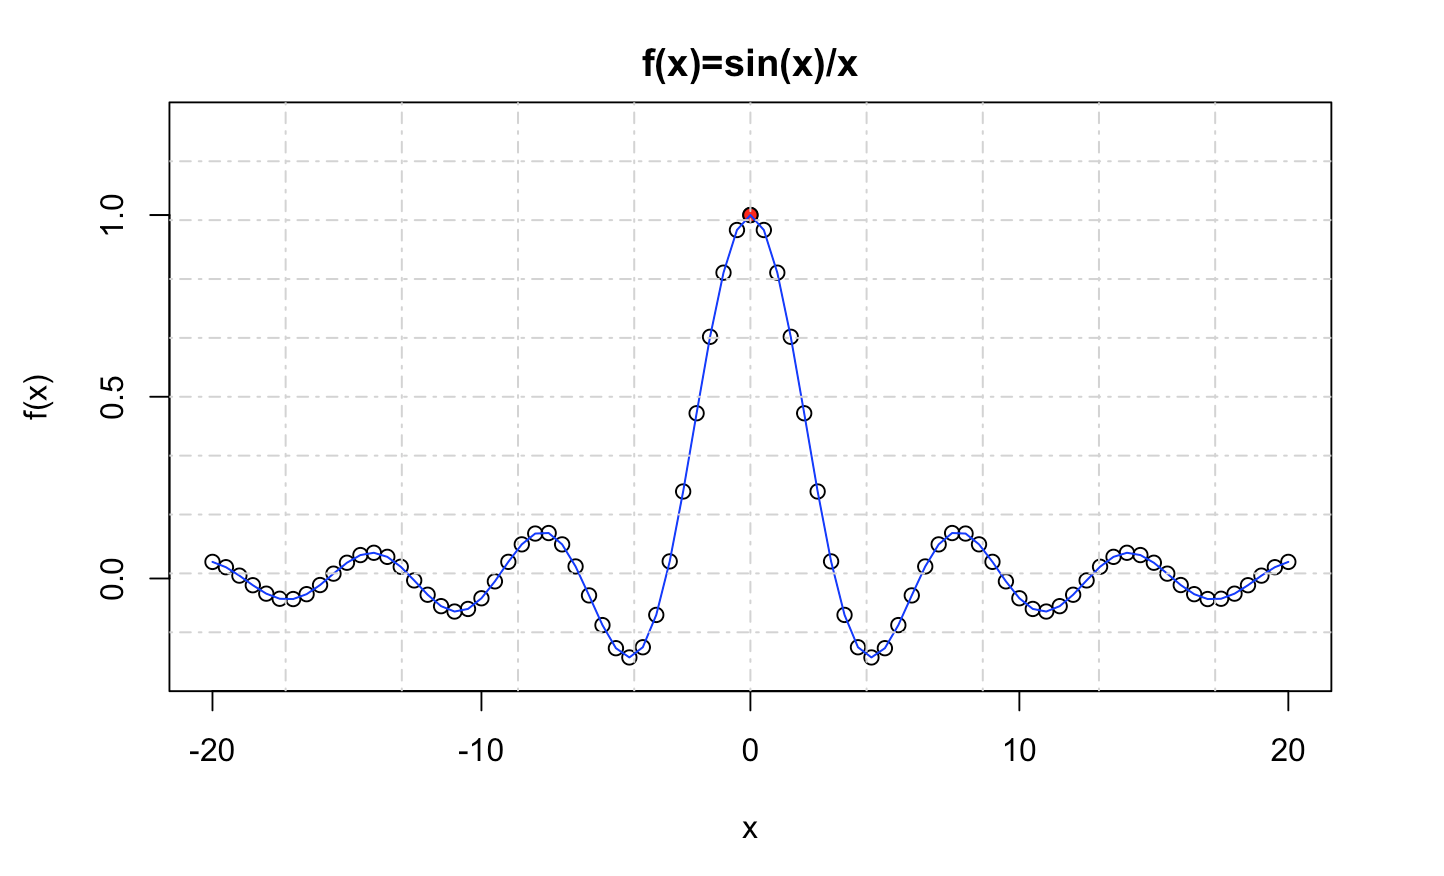
\includegraphics{sinxx.png}

\begin{Shaded}
\begin{Highlighting}[]
\CommentTok{#solución:}
\end{Highlighting}
\end{Shaded}

\begin{center}\rule{0.5\linewidth}{0.5pt}\end{center}

\hypertarget{factor}{%
\section{Factor}\label{factor}}

\hypertarget{create-factor}{%
\subsection{Create Factor}\label{create-factor}}

\hypertarget{unordered}{%
\subsubsection{Unordered}\label{unordered}}

\begin{Shaded}
\begin{Highlighting}[]
\NormalTok{sex.v <-}\StringTok{ }\KeywordTok{c}\NormalTok{(}\StringTok{'M'}\NormalTok{, }\StringTok{'F'}\NormalTok{, }\StringTok{'F'}\NormalTok{, }\StringTok{'M'}\NormalTok{, }\StringTok{'M'}\NormalTok{, }\StringTok{'F'}\NormalTok{)}
\NormalTok{sex.f <-}\StringTok{ }\KeywordTok{factor}\NormalTok{(sex.v) }\CommentTok{# unordered}
\NormalTok{sex.w <-}\StringTok{ }\KeywordTok{as.character}\NormalTok{(sex.f) }\CommentTok{# restore}
\end{Highlighting}
\end{Shaded}

\hypertarget{ordered}{%
\subsubsection{Ordered}\label{ordered}}

\begin{Shaded}
\begin{Highlighting}[]
\NormalTok{size.v <-}\StringTok{ }\KeywordTok{c}\NormalTok{(}\StringTok{'S'}\NormalTok{, }\StringTok{'L'}\NormalTok{, }\StringTok{'M'}\NormalTok{, }\StringTok{'L'}\NormalTok{, }\StringTok{'S'}\NormalTok{, }\StringTok{'M'}\NormalTok{)}
\NormalTok{size.f <-}\StringTok{ }\KeywordTok{factor}\NormalTok{(size.v, }\DataTypeTok{ordered=}\OtherTok{TRUE}\NormalTok{)}
\CommentTok{# ordered L < M < S from underlying type}
\end{Highlighting}
\end{Shaded}

\hypertarget{ordered-where-we-set-the-order}{%
\subsubsection{Ordered, where we set the
order}\label{ordered-where-we-set-the-order}}

\begin{Shaded}
\begin{Highlighting}[]
\NormalTok{size.lvls <-}\StringTok{ }\KeywordTok{c}\NormalTok{(}\StringTok{'S'}\NormalTok{, }\StringTok{'M'}\NormalTok{, }\StringTok{'L'}\NormalTok{) }\CommentTok{# set order}
\NormalTok{size.f <-}\StringTok{ }\KeywordTok{factor}\NormalTok{(size.v, }\DataTypeTok{levels=}\NormalTok{size.lvls, }\DataTypeTok{ordered=}\OtherTok{TRUE}\NormalTok{)}
\CommentTok{# above: ordered (low to high) by levels}
\end{Highlighting}
\end{Shaded}

\hypertarget{ordered-with-levels-and-labels}{%
\subsubsection{Ordered with levels and
labels}\label{ordered-with-levels-and-labels}}

\begin{Shaded}
\begin{Highlighting}[]
\NormalTok{levels <-}\StringTok{ }\KeywordTok{c}\NormalTok{(}\DecValTok{1}\NormalTok{, }\DecValTok{2}\NormalTok{, }\DecValTok{3}\NormalTok{, }\DecValTok{99}\NormalTok{) }\CommentTok{# from codesheet}
\NormalTok{labels <-}\StringTok{ }\KeywordTok{c}\NormalTok{(}\StringTok{'Love'}\NormalTok{,}\StringTok{'Neutral'}\NormalTok{,}\StringTok{'Hate'}\NormalTok{,}\OtherTok{NA}\NormalTok{)}
\NormalTok{data.v <-}\StringTok{ }\KeywordTok{c}\NormalTok{(}\DecValTok{1}\NormalTok{, }\DecValTok{2}\NormalTok{, }\DecValTok{3}\NormalTok{, }\DecValTok{99}\NormalTok{, }\DecValTok{1}\NormalTok{, }\DecValTok{2}\NormalTok{, }\DecValTok{1}\NormalTok{, }\DecValTok{2}\NormalTok{, }\DecValTok{99}\NormalTok{)}
\NormalTok{data.f <-}\StringTok{ }\KeywordTok{factor}\NormalTok{(data.v, }\DataTypeTok{levels=}\NormalTok{levels)}
\NormalTok{data.f <-}\StringTok{ }\KeywordTok{factor}\NormalTok{(data.v, }\DataTypeTok{levels=}\NormalTok{levels,}\DataTypeTok{labels=}\NormalTok{labels)}
\CommentTok{# levels: input - how factor() reads in}
\CommentTok{# labels: output - how factor() puts out}
\CommentTok{# Note: if specified, labels become the internal reference and coding frame}
\end{Highlighting}
\end{Shaded}

\hypertarget{managing-factors}{%
\subsection{Managing Factors}\label{managing-factors}}

\hypertarget{get-levels}{%
\subsubsection{Get Levels}\label{get-levels}}

\begin{Shaded}
\begin{Highlighting}[]
\NormalTok{f <-}\StringTok{ }\KeywordTok{factor}\NormalTok{(}\KeywordTok{c}\NormalTok{(}\StringTok{"a"}\NormalTok{,}\StringTok{"b"}\NormalTok{,}\StringTok{"c"}\NormalTok{)) }\CommentTok{# example data}
\KeywordTok{levels}\NormalTok{(f) }\CommentTok{# -> get all levels}
\end{Highlighting}
\end{Shaded}

\begin{verbatim}
## [1] "a" "b" "c"
\end{verbatim}

\begin{Shaded}
\begin{Highlighting}[]
\KeywordTok{levels}\NormalTok{(f)[}\DecValTok{1}\NormalTok{] }\CommentTok{# -> get a specific level}
\end{Highlighting}
\end{Shaded}

\begin{verbatim}
## [1] "a"
\end{verbatim}

Get get all levels of \texttt{s} factor.

\begin{itemize}
\tightlist
\item
  Rename the factors so that they start with a capital letter.
\item
  Test existence of a level ``Divorced''.
\item
  Add the level ``Divorced''
\item
  Modify second element to ``Divorced''.
\end{itemize}

\begin{Shaded}
\begin{Highlighting}[]
\NormalTok{s <-}\StringTok{ }\KeywordTok{factor}\NormalTok{(}\KeywordTok{c}\NormalTok{(}\StringTok{"single"}\NormalTok{, }\StringTok{"married"}\NormalTok{, }\StringTok{"married"}\NormalTok{, }\StringTok{"single"}\NormalTok{));}
\NormalTok{s}
\end{Highlighting}
\end{Shaded}

\begin{verbatim}
## [1] single  married married single 
## Levels: married single
\end{verbatim}

\begin{Shaded}
\begin{Highlighting}[]
\CommentTok{#solution}
\end{Highlighting}
\end{Shaded}

Use the \texttt{cut} function to create the \texttt{age} ordered factor
with 3 levels from \texttt{v} vector.

\begin{itemize}
\tightlist
\item
  Change de levels to ``young'' \textless{} ``adult'' \textless{}
  ``older''.
\item
  Select the values of \texttt{v} that match \texttt{age} less than
  ``older''.
\end{itemize}

\begin{Shaded}
\begin{Highlighting}[]
\NormalTok{v<-}\KeywordTok{c}\NormalTok{(40L, 35L, 69L, 74L, 38L, 58L, 13L, 27L, 17L, 68L, 21L, 80L, }
\NormalTok{42L, 19L, 29L, 52L, 65L, 40L, 80L, 23L, 59L, 78L, 37L, 38L, 76L, }
\NormalTok{75L, 3L, 22L, 29L, 29L)}

\CommentTok{#solution}
\end{Highlighting}
\end{Shaded}

\hypertarget{plot-factors}{%
\subsection{Plot Factors}\label{plot-factors}}

\begin{Shaded}
\begin{Highlighting}[]
\NormalTok{v<-}\KeywordTok{c}\NormalTok{(}\StringTok{"L"}\NormalTok{, }\StringTok{"M"}\NormalTok{, }\StringTok{"M"}\NormalTok{, }\StringTok{"L"}\NormalTok{, }\StringTok{"M"}\NormalTok{, }\StringTok{"L"}\NormalTok{, }\StringTok{"M"}\NormalTok{, }\StringTok{"L"}\NormalTok{, }\StringTok{"L"}\NormalTok{, }\StringTok{"L"}\NormalTok{, }\StringTok{"M"}\NormalTok{, }\StringTok{"M"}\NormalTok{, }
\StringTok{"L"}\NormalTok{, }\StringTok{"M"}\NormalTok{, }\StringTok{"S"}\NormalTok{, }\StringTok{"L"}\NormalTok{, }\StringTok{"M"}\NormalTok{, }\StringTok{"S"}\NormalTok{, }\StringTok{"M"}\NormalTok{, }\StringTok{"L"}\NormalTok{, }\StringTok{"M"}\NormalTok{, }\StringTok{"L"}\NormalTok{, }\StringTok{"S"}\NormalTok{, }\StringTok{"S"}\NormalTok{, }\StringTok{"M"}\NormalTok{, }
\StringTok{"L"}\NormalTok{, }\StringTok{"L"}\NormalTok{, }\StringTok{"M"}\NormalTok{, }\StringTok{"M"}\NormalTok{, }\StringTok{"M"}\NormalTok{)}
\KeywordTok{plot}\NormalTok{(}\KeywordTok{factor}\NormalTok{(v)) }\CommentTok{# unordered}
\end{Highlighting}
\end{Shaded}

\includegraphics{Ejercicios_SesionR3_files/figure-latex/unnamed-chunk-14-1.pdf}

\begin{Shaded}
\begin{Highlighting}[]
\KeywordTok{plot}\NormalTok{(}\KeywordTok{factor}\NormalTok{(v, }\DataTypeTok{levels=}\KeywordTok{c}\NormalTok{(}\StringTok{'S'}\NormalTok{, }\StringTok{'M'}\NormalTok{, }\StringTok{'L'}\NormalTok{), }\DataTypeTok{ordered=}\OtherTok{TRUE}\NormalTok{)) }\CommentTok{#ordered}
\end{Highlighting}
\end{Shaded}

\includegraphics{Ejercicios_SesionR3_files/figure-latex/unnamed-chunk-14-2.pdf}

Modifica el gráfico anterior obtenido del factor(v) para obtener el
siguiente resultado.

\begin{Shaded}
\begin{Highlighting}[]
\CommentTok{#solución: }
\end{Highlighting}
\end{Shaded}

\begin{center}\rule{0.5\linewidth}{0.5pt}\end{center}

\hypertarget{list}{%
\section{List}\label{list}}

\hypertarget{lists-creation}{%
\subsection{Lists Creation}\label{lists-creation}}

\begin{Shaded}
\begin{Highlighting}[]
\NormalTok{l1 <-}\StringTok{ }\KeywordTok{list}\NormalTok{(}\StringTok{'cat'}\NormalTok{, }\DecValTok{5}\NormalTok{, }\DecValTok{1}\OperatorTok{:}\DecValTok{10}\NormalTok{, }\OtherTok{FALSE}\NormalTok{) }\CommentTok{# unnamed }
\NormalTok{l2 <-}\StringTok{ }\KeywordTok{list}\NormalTok{(}\DataTypeTok{x=}\StringTok{'dog'}\NormalTok{, }\DataTypeTok{y=}\DecValTok{5}\OperatorTok{+}\NormalTok{2i, }\DataTypeTok{z=}\DecValTok{3}\OperatorTok{:}\DecValTok{8}\NormalTok{) }\CommentTok{# named }
\NormalTok{l3 <-}\StringTok{ }\KeywordTok{c}\NormalTok{(l1, l2) }\CommentTok{# one list partially named }
\NormalTok{l4 <-}\StringTok{ }\KeywordTok{list}\NormalTok{(l1, l2) }\CommentTok{# a list of 2 lists}
\end{Highlighting}
\end{Shaded}

\hypertarget{indexing-examples}{%
\subsection{Indexing examples}\label{indexing-examples}}

\begin{Shaded}
\begin{Highlighting}[]
\NormalTok{j <-}\StringTok{ }\KeywordTok{list}\NormalTok{(}\DataTypeTok{a=}\StringTok{'cat'}\NormalTok{, }\DataTypeTok{b=}\DecValTok{5}\NormalTok{, }\DataTypeTok{c=}\OtherTok{FALSE}\NormalTok{)}
\NormalTok{x1 <-}\StringTok{ }\NormalTok{j}\OperatorTok{$}\NormalTok{a }\CommentTok{# puts 1-item char vec 'cat' in x}
\NormalTok{x2 <-}\StringTok{ }\NormalTok{j[[}\StringTok{'a'}\NormalTok{]] }\CommentTok{# much the same as above}
\NormalTok{x3 <-}\StringTok{ }\NormalTok{j[}\StringTok{'a'}\NormalTok{] }\CommentTok{# puts 1-item list 'cat' in x}
\NormalTok{x4 <-}\StringTok{ }\NormalTok{j[[}\DecValTok{1}\NormalTok{]] }\CommentTok{# 1-item char vec 'cat' in x}
\NormalTok{x5 <-}\StringTok{ }\NormalTok{j[}\DecValTok{1}\NormalTok{] }\CommentTok{# puts 1-item list 'cat' in x}
\end{Highlighting}
\end{Shaded}

Dada la lista \texttt{l} dada:

\begin{itemize}
\tightlist
\item
  Añade el vector ``n'' en la sexta posición de la lista.
\item
  ¿Qué ha pasado con el quinto elemento de la lista?
\item
  Añade el vector ``w'' en el elemento ``k'' de la lista.
\item
  Cambia el contenido del la posición ``w'' al valor ``e''
\end{itemize}

\begin{Shaded}
\begin{Highlighting}[]
\NormalTok{l <-}\StringTok{ }\KeywordTok{list}\NormalTok{(}\DataTypeTok{x=}\StringTok{'a'}\NormalTok{, }\DataTypeTok{y=}\StringTok{'b'}\NormalTok{, }\DataTypeTok{z=}\StringTok{'c'}\NormalTok{, }\DataTypeTok{t=}\StringTok{'d'}\NormalTok{)}

\CommentTok{#solucion }
\end{Highlighting}
\end{Shaded}

The \texttt{vocals} list has a sample of the vowels of different
supports: * How many items does the list have? * Which item is longer?
uses the \texttt{str} instruction to get information about its content.
* Turn the \texttt{notebook} item into the \texttt{f.notebook} factor
and plot it.

\begin{Shaded}
\begin{Highlighting}[]
\NormalTok{vocals<-}\KeywordTok{list}\NormalTok{(}\DataTypeTok{story =} \KeywordTok{c}\NormalTok{(}\StringTok{"e"}\NormalTok{, }\StringTok{"e"}\NormalTok{, }\StringTok{"e"}\NormalTok{, }\StringTok{"e"}\NormalTok{, }\StringTok{"a"}\NormalTok{, }\StringTok{"e"}\NormalTok{, }\StringTok{"o"}\NormalTok{, }
\StringTok{"o"}\NormalTok{, }\StringTok{"o"}\NormalTok{, }\StringTok{"a"}\NormalTok{), }\DataTypeTok{poetry =} \KeywordTok{c}\NormalTok{(}\StringTok{"e"}\NormalTok{, }\StringTok{"e"}\NormalTok{, }\StringTok{"i"}\NormalTok{, }\StringTok{"e"}\NormalTok{, }\StringTok{"e"}\NormalTok{), }\DataTypeTok{book =} \KeywordTok{c}\NormalTok{(}\StringTok{"e"}\NormalTok{, }
\StringTok{"e"}\NormalTok{, }\StringTok{"e"}\NormalTok{, }\StringTok{"o"}\NormalTok{, }\StringTok{"e"}\NormalTok{, }\StringTok{"o"}\NormalTok{, }\StringTok{"u"}\NormalTok{, }\StringTok{"o"}\NormalTok{, }\StringTok{"e"}\NormalTok{, }\StringTok{"e"}\NormalTok{, }\StringTok{"a"}\NormalTok{, }\StringTok{"i"}\NormalTok{, }\StringTok{"a"}\NormalTok{, }\StringTok{"u"}\NormalTok{, }
\StringTok{"e"}\NormalTok{, }\StringTok{"a"}\NormalTok{, }\StringTok{"o"}\NormalTok{, }\StringTok{"u"}\NormalTok{, }\StringTok{"e"}\NormalTok{, }\StringTok{"e"}\NormalTok{, }\StringTok{"a"}\NormalTok{, }\StringTok{"e"}\NormalTok{, }\StringTok{"a"}\NormalTok{, }\StringTok{"o"}\NormalTok{, }\StringTok{"e"}\NormalTok{, }\StringTok{"a"}\NormalTok{, }\StringTok{"a"}\NormalTok{, }
\StringTok{"e"}\NormalTok{, }\StringTok{"o"}\NormalTok{, }\StringTok{"e"}\NormalTok{, }\StringTok{"u"}\NormalTok{, }\StringTok{"o"}\NormalTok{, }\StringTok{"u"}\NormalTok{, }\StringTok{"a"}\NormalTok{, }\StringTok{"o"}\NormalTok{, }\StringTok{"u"}\NormalTok{, }\StringTok{"i"}\NormalTok{, }\StringTok{"a"}\NormalTok{, }\StringTok{"a"}\NormalTok{, }\StringTok{"u"}\NormalTok{, }
\StringTok{"a"}\NormalTok{, }\StringTok{"a"}\NormalTok{, }\StringTok{"e"}\NormalTok{, }\StringTok{"u"}\NormalTok{, }\StringTok{"a"}\NormalTok{, }\StringTok{"e"}\NormalTok{, }\StringTok{"a"}\NormalTok{, }\StringTok{"e"}\NormalTok{, }\StringTok{"a"}\NormalTok{, }\StringTok{"a"}\NormalTok{), }\DataTypeTok{notebook =} \KeywordTok{c}\NormalTok{(}\StringTok{"a"}\NormalTok{, }
\StringTok{"o"}\NormalTok{, }\StringTok{"e"}\NormalTok{, }\StringTok{"e"}\NormalTok{, }\StringTok{"e"}\NormalTok{, }\StringTok{"a"}\NormalTok{, }\StringTok{"a"}\NormalTok{, }\StringTok{"i"}\NormalTok{, }\StringTok{"e"}\NormalTok{, }\StringTok{"a"}\NormalTok{, }\StringTok{"u"}\NormalTok{, }\StringTok{"e"}\NormalTok{, }\StringTok{"e"}\NormalTok{, }\StringTok{"i"}\NormalTok{, }
\StringTok{"a"}\NormalTok{, }\StringTok{"e"}\NormalTok{, }\StringTok{"e"}\NormalTok{, }\StringTok{"o"}\NormalTok{, }\StringTok{"e"}\NormalTok{, }\StringTok{"e"}\NormalTok{), }\DataTypeTok{booklet =} \KeywordTok{c}\NormalTok{(}\StringTok{"e"}\NormalTok{, }\StringTok{"e"}\NormalTok{, }\StringTok{"o"}\NormalTok{, }\StringTok{"i"}\NormalTok{, }
\StringTok{"i"}\NormalTok{, }\StringTok{"o"}\NormalTok{, }\StringTok{"a"}\NormalTok{, }\StringTok{"i"}\NormalTok{, }\StringTok{"i"}\NormalTok{, }\StringTok{"a"}\NormalTok{, }\StringTok{"i"}\NormalTok{, }\StringTok{"e"}\NormalTok{, }\StringTok{"i"}\NormalTok{, }\StringTok{"o"}\NormalTok{, }\StringTok{"a"}\NormalTok{, }\StringTok{"a"}\NormalTok{, }\StringTok{"o"}\NormalTok{, }
\StringTok{"o"}\NormalTok{, }\StringTok{"o"}\NormalTok{, }\StringTok{"e"}\NormalTok{, }\StringTok{"o"}\NormalTok{, }\StringTok{"a"}\NormalTok{, }\StringTok{"o"}\NormalTok{, }\StringTok{"i"}\NormalTok{, }\StringTok{"o"}\NormalTok{, }\StringTok{"e"}\NormalTok{, }\StringTok{"e"}\NormalTok{, }\StringTok{"i"}\NormalTok{, }\StringTok{"a"}\NormalTok{, }\StringTok{"u"}
\NormalTok{))}

\CommentTok{# solution}
\end{Highlighting}
\end{Shaded}

Create a \texttt{hotel} list containing information about people. Enter
the name, surname and age of the following actors: * Rachel Weisz, age=
48 * Gerard Butler age=48

\begin{Shaded}
\begin{Highlighting}[]
\NormalTok{hotel<-}\KeywordTok{list}\NormalTok{()}

\CommentTok{#solution}
\end{Highlighting}
\end{Shaded}

\begin{center}\rule{0.5\linewidth}{0.5pt}\end{center}

\hypertarget{generaciuxf3n-de-guiuxf3n-de-ejercicios-completos}{%
\section{Generación de Guión de Ejercicios
Completos}\label{generaciuxf3n-de-guiuxf3n-de-ejercicios-completos}}

Compila este documento en formato HTML y genera el documento de los
ejercicios (¡ahora completados!) de la sesión de Introducción al
Lenguaje R.

\end{document}
